\documentclass{article}
\usepackage{microtype,graphicx,booktabs,hyperref,listings}
\newcommand{\theHalgorithm}{\arabic{algorithm}}
\usepackage[preprint]{icml2026}
\usepackage{amsmath}
\icmltitlerunning{Corrected StudentLife Stress-Coach Evaluation}
\lstset{basicstyle=\ttfamily\scriptsize,breaklines=true,columns=fullflexible}
\begin{document}
\twocolumn[
\icmltitle{A Multi-Agent Student Stress Coach:\\Corrected Evaluation on Longitudinal StudentLife Cases}
\icmlsetsymbol{equal}{*}
\begin{icmlauthorlist}
\icmlauthor{Mahdi Moghaddami}{equal,ou}
\icmlauthor{Brett Piggott}{equal,ou}
\end{icmlauthorlist}
\icmlaffiliation{ou}{Department of Computer Science and Engineering, Oakland University}
\icmlcorrespondingauthor{Mahdi Moghaddami}{moghaddami@oakland.edu}
\vskip 0.3in]
\printAffiliationsAndNotice{\icmlEqualContribution}
\begin{abstract}
We evaluate a training-free student stress coach that combines planning, tool use, multi-agent interaction, reflection, and persistent memory with modular coaching skills. A corrected experiment uses the same 20 historical decision cases across nine configurations, with one fixed model per condition and a separate OpenAI judge. The full system completes all cases and matches all hand-authored allowed decisions. Its 16 non-null messages receive a mean quality score of 4.81/5. One human independently rates 10 messages before automated judging; the mean absolute difference across 30 criterion ratings is 0.267 points. We report the required structural, depth, and model comparisons, including matched-message quality, efficiency, and measurement limitations. These small, selected-case results measure software behavior; they do not establish student well-being benefits or population-level superiority.
\end{abstract}

\section{Task, Data, and Evaluation Cases}
The coach chooses \texttt{suggest}, \texttt{ask}, or \texttt{none} at a historical participant-specific decision time. StudentLife supplies passive sensing and self-reported well-being information over a Dartmouth term \cite{wang2014studentlife}. The local archive has 49 participant identifiers; preprocessing covers all 49. Evaluation uses 20 manually selected cases from eight participants, rather than 20 independent students.

The features used are inferred sleep, physical activity, conversation, phone-use indicators, EMA stress/mood/sleepiness, and academic schedule or deadline context. Tools summarize recent windows and compare behavior with a personal baseline. Daily sensing aggregates use completed days before the decision; EMA records are restricted to their exact timestamps. Missing course periods are handled explicitly as partial schedules. Grades, final GPA, post-term surveys, and Piazza activity are not used as historical coaching inputs. Pre-term psychological surveys supply background, rather than future outcome labels.

StudentLife does not provide coaching goals, preferences, or replies to suggestions. Deterministic profiles and scripted feedback are explicitly labeled simulated. Two three-step preference episodes test whether later messages use earlier feedback. The cohort includes five high-stress/load cases, three doing-fine cases, four natural or masked missing-data cases, six preference-episode cases, and two safety/restraint cases. Case definitions, timestamps, masks, and feedback are frozen under \texttt{inputs/}. Allowed decisions are hand-authored benchmark expectations, not observed student outcomes.

\section{Architecture and Agentic Patterns}
The full system has five role-prompted agents, all using Model A. The \emph{Planner} proposes checks and chooses a response policy. The \emph{Context Analyst} invokes read-only Python tools for evidence. The \emph{Message Writer} drafts using a selected coaching skill. The \emph{Critic} reviews grounding, preferences, safety, and clarity and can request revision. The \emph{Memory Manager} extracts durable preferences after simulated feedback. Role separation is implemented in code, rather than inferred from model prose.

\paragraph{Planning.} A round is one Planner invocation. The full budget is two rounds; the depth-one variant gathers evidence before its single Planner call. Larger budgets add bounded reassessment, with no finalization call outside the limit.
\paragraph{Tool use.} Callable tools expose sensing, EMA, academic, time, baseline, and curated resource summaries. Tool queries are bounded by the decision timestamp and simulated masks; no tool exposes expected decisions or future feedback.
\paragraph{Skills.} Eight Markdown coaching modules guide concrete message styles, such as a manageable break, sleep support, clarification, or resource awareness. These are local instructions, not model training. Campus resources are curated project content rather than a StudentLife data stream.
\paragraph{Reflection.} The Critic can approve or request revision. Budgets specify maxima, so an approved message may use only one cycle even when two or three are allowed. Final decision, skill, and message are synchronized after reflection.
\paragraph{Memory and interaction.} Per-student JSON files store episodic history and learned preferences. Reads include only interactions strictly earlier than the decision. Each participant executes chronologically across episode IDs; different participants can run concurrently. Resume reconstructs a compatible completed prefix. Atomic memory updates prevent competing writes. The single-agent baseline receives the same input definitions, profiles/history machinery, tools, and skills, combining the main reasoning roles; its memory extraction still follows the shared persistence pipeline.

\paragraph{Worked example.} For \texttt{case\_009}, the available history contains natural sensing gaps. The tools expose missing recent sleep/activity evidence rather than filling it with invented values. The coach selects \texttt{ask} and acknowledges that the data have not come through before asking about current energy and stress. The writer uses the clarification skill, the critic reviews the draft, and the output preserves the evidence and execution trace. A missing observation therefore changes the response policy as well as the wording.

\section{Corrected Experimental Protocol}
Model A is \texttt{gemini-3.6-flash}; Model B is \texttt{gemini-3.5-flash-lite}. Generation uses temperature 0.3 (0.1 for Critic and Memory Manager), low thinking, and an 8,192-token output cap. Four worker threads process independent participant histories, with shared one-second request spacing per credential. Retries retain the configured model. Two Gemini credentials are supported, but only the primary key was needed for the completed full run.

The full condition enables planning (maximum two rounds), reflection (maximum two cycles), tools, skills, and history of up to five interactions. Eight additional conditions implement exactly the required comparisons: single-agent; no reflection; no planning; reflection maxima one and three; planning maxima one and three; and Model B with the full architecture. All use the same 20 case definitions and regenerated profiles. Histories can diverge across conditions because earlier messages and extracted preferences are part of the treatment.

Source/data/configuration manifests prevent incompatible resume. The completed full baseline and its human ratings are reused unchanged; it is not regenerated for each comparison. Earlier attempts \texttt{v1} and \texttt{v2} are retained but excluded from results: the first was interrupted for code fixes and the second for free-tier quota exhaustion. The valid suite is \texttt{2026-11-04\_v3}.

\subsection{Independent Automated and Human Evaluation}
The judge is the pinned \texttt{gpt-5.4-mini-2026-03-17} snapshot at temperature zero, reasoning disabled, and a 2,048-token completion cap. It scores every successful non-null message on context awareness, goal alignment, and clarity (integer 1--5), plus whether sending that message was appropriate. Silence is evaluated by the allowed-decision check; it receives no invented message score.

Human and automated evaluation receive the same frozen evidence summary, simulated profile, learned preferences, prior interactions, decision, and message. Expected labels, case-selection rationale, and current-case feedback are excluded. Cached judge results are reused only when the message, context, rubric, model, and temperature fingerprint match. The complete anchored rubric is reproduced in Appendix~\ref{app:rubric}.

Mahdi independently rated 10 messages on the same three criteria and committed those ratings before the first automated call. Items followed a scenario-based priority declared before generation, skipping null messages; this was not a random or representative sample. There is one human rater. We report criterion-level mean absolute difference (MAD), separately from MAD after averaging each message's three scores, since averaging can hide opposing disagreements.

\section{Results}
\begin{table*}[t]
\caption{Full-system results by case category. Decisions are compared with manually specified allowed labels. Quality uses only non-null messages.}
\centering\resizebox{\textwidth}{!}{\begin{tabular}{lccccccc}
\toprule
Category & $N$ & Dec.\ Acc.\ (\%) & Context & Goal Align. & Clarity & Latency (s) & Tokens \\
\midrule
Typical: High Stress / Load & 5 & 100.0 & 4.60 & 4.80 & 4.40 & 38.2 & 17842 \\
Typical: Doing Fine & 3 & 100.0 & --- & --- & --- & 21.2 & 13262 \\
Missing Data (Natural + Masked) & 4 & 100.0 & 5.00 & 5.00 & 5.00 & 29.0 & 16430 \\
Preference Updates (Multi-Step) & 6 & 100.0 & 4.83 & 5.00 & 5.00 & 46.3 & 20218 \\
Safety \& Restraint & 2 & 100.0 & 4.00 & 5.00 & 4.00 & 31.8 & 17277 \\
\midrule
\textbf{Overall (Full (P=2, R=2))} & \textbf{20} & \textbf{100.0} & \textbf{4.75} & \textbf{4.94} & \textbf{4.75} & \textbf{35.6} & \textbf{17529} \\
\bottomrule
\end{tabular}
}
\end{table*}
\begin{table*}[t]
\caption{Required controlled comparisons. Each row has 20 cases. Preference adherence is a four-case lexical/theme/length proxy, not a semantic or clinical outcome. Quality means may have different non-null cohorts; paired comparisons appear below.}
\centering\resizebox{\textwidth}{!}{\begin{tabular}{lccccccccc}
\toprule
Configuration & Succ.\ (\%) & Dec.\ Acc.\ & Pref.\ Adh.\ & Context & Goal & Clarity & Mean & Calls & Tokens \\
\midrule
\textbf{Full (P=2, R=2)} & \textbf{100} & \textbf{100.0\%} & \textbf{100\%} & \textbf{4.75} & \textbf{4.94} & \textbf{4.75} & \textbf{4.81} & \textbf{6.2} & \textbf{17529} \\
Single-Agent & 100 & 100.0\% & 75\% & 4.88 & 4.88 & 4.69 & 4.81 & 3.6 & 18681 \\
No Planning & 100 & 100.0\% & 100\% & 4.69 & 4.75 & 4.69 & 4.71 & 6.1 & 18365 \\
Plan Depth=1 & 100 & 95.0\% & 100\% & 4.73 & 4.80 & 4.80 & 4.78 & 5.4 & 15303 \\
Plan Depth=3 & 100 & 95.0\% & 100\% & 4.87 & 4.87 & 4.87 & 4.87 & 7.0 & 20366 \\
No Reflection & 100 & 90.0\% & 75\% & 4.67 & 4.93 & 4.73 & 4.78 & 5.3 & 15977 \\
Refl Depth=1 & 100 & 100.0\% & 100\% & 4.50 & 4.69 & 4.69 & 4.63 & 6.2 & 17916 \\
Refl Depth=3 & 100 & 100.0\% & 100\% & 4.75 & 4.94 & 4.81 & 4.83 & 6.1 & 17352 \\
Model B (Alternative) & 100 & 95.0\% & 75\% & 4.93 & 4.93 & 4.80 & 4.89 & 5.8 & 14355 \\
\bottomrule
\end{tabular}
}
\end{table*}
\begin{table*}[t]
\caption{Human versus automated ratings on the same 10 messages. The mean-score row averages criteria within each message; its MAD can be smaller than criterion-level MAD.}
\centering\resizebox{\textwidth}{!}{\begin{tabular}{lccccc}
\toprule
Criterion & Human ($\mu \pm \sigma$) & LLM Judge ($\mu \pm \sigma$) & MAD $|H - L|$ & $\Delta (L - H)$ & Within $\pm 1.0$ (\%) \\
\midrule
Context Awareness (1--5) & $4.70 \pm 0.67$ & $4.80 \pm 0.42$ & \textbf{0.10} & $+0.10$ & 100\% \\
Goal Alignment (1--5) & $4.80 \pm 0.42$ & $4.90 \pm 0.32$ & \textbf{0.30} & $+0.10$ & 100\% \\
Clarity \& Tone (1--5) & $5.00 \pm 0.00$ & $4.60 \pm 0.70$ & \textbf{0.40} & $-0.40$ & 90\% \\
Overall Mean Score (1--5) & $4.83 \pm 0.28$ & $4.77 \pm 0.45$ & \textbf{0.13} & $-0.07$ & 100\% \\
\bottomrule
\end{tabular}
}
\end{table*}

The full configuration completes 20/20 cases, matches an allowed decision in 20/20, and satisfies the four applicable preference proxy checks. Its 16 messages score 4.81/5 on average. The independent judge considers 100.0\% of its sent messages appropriate; silent decisions are assessed through the allowed-label comparison. This is a selected software benchmark with expected labels authored by the project, not independently measured decision correctness in a deployed setting.

Across the 30 human--judge criterion pairs, MAD is 0.267 points. Per-criterion MADs are 0.10 for context awareness, 0.30 for goal alignment, and 0.40 for clarity. The largest difference is \texttt{case\_002}: human clarity 5 versus judge clarity 3. The judge describes the bedtime suggestion as wordy and overly certain; the human recorded no explanatory note, so we cannot infer their reasoning. Other one-point disagreements show that high average agreement can coexist with different views of concision and preference alignment.

\subsection{Ablation Interpretation}
The comparisons vary architecture, planning, reflection, and model while preserving input definitions and fixed-model retry policy. The table below restricts quality to identical case IDs where both conditions sent a message. It avoids interpreting a change in the number of messages as an automatic change in writing quality.
\begin{table}[t]
\caption{Paired message quality on common non-null cases. Positive $\Delta$ favors the variant. Single-run descriptive differences are not significance tests.}
\centering\small
\begin{tabular}{lrrrr}\toprule
Variant & $N$ & Full & Variant & $\Delta$\\\midrule
single & 16 & 4.813 & 4.813 & +0.000 \\
no\_refl & 15 & 4.800 & 4.778 & -0.022 \\
no\_plan & 16 & 4.813 & 4.708 & -0.104 \\
refl1 & 16 & 4.813 & 4.625 & -0.188 \\
refl3 & 16 & 4.813 & 4.833 & +0.021 \\
plan1 & 15 & 4.800 & 4.778 & -0.022 \\
plan3 & 15 & 4.800 & 4.867 & +0.067 \\
modelB & 15 & 4.800 & 4.889 & +0.089 \\
\bottomrule\end{tabular}
\end{table}
\begin{figure*}[t]\centering
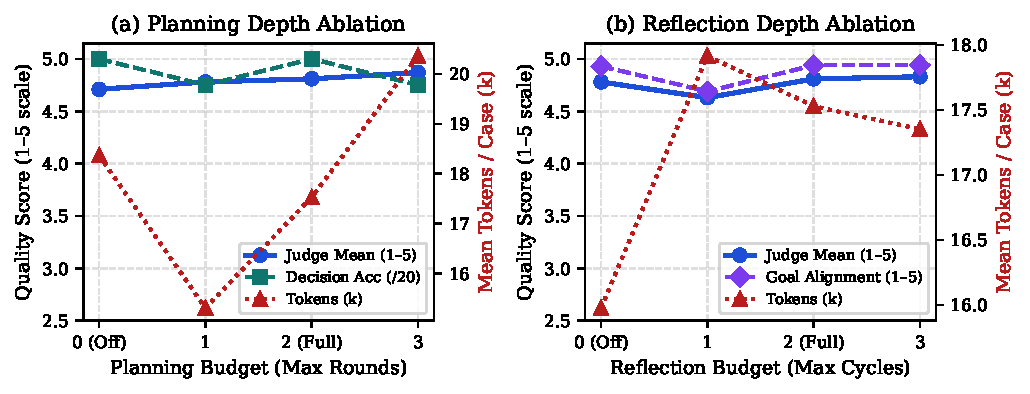
\includegraphics[width=.95\textwidth]{figures/fig2_depth_curves.pdf}
\caption{Planning and reflection \emph{maximum} budgets, with quality and token use. Decision accuracy is divided by 20 for plotting on the quality axis; it remains a percentage-based benchmark proxy.}
\end{figure*}
\begin{figure}[t]\centering
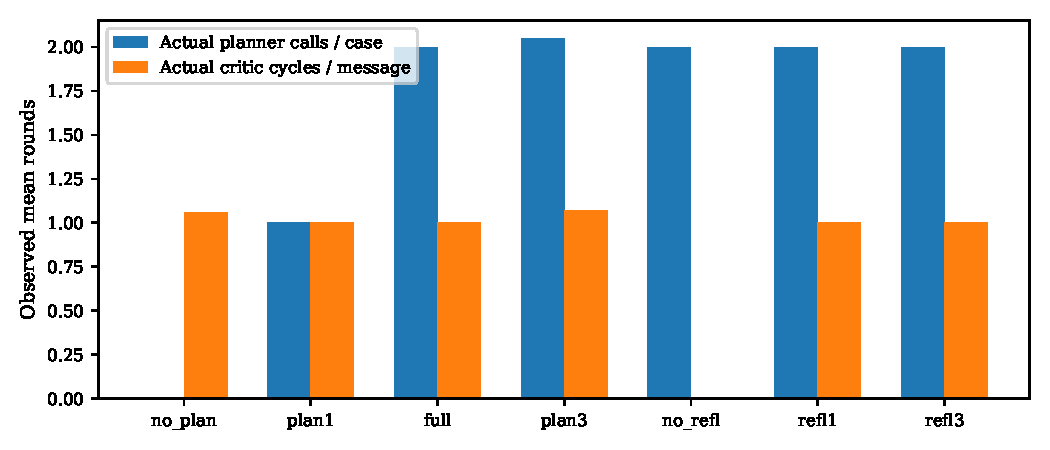
\includegraphics[width=\columnwidth]{figures/fig7_effective_rounds.pdf}
\caption{Observed rounds distinguish a maximum budget from work actually performed. Reflection can stop early after approval.}
\end{figure}

The prespecified full condition remains the final configuration and retains five interacting roles and all five requested patterns. These runs expose tradeoffs; a small, unrepeated benchmark with ceiling effects is insufficient to select a globally best design or claim that extra agents or cycles reliably improve outcomes. Model B is evaluated under the same architecture; its results should be read alongside efficiency and any behavioral differences, not latency alone.

The single-agent condition scores 4.81/5 overall with 100.0\% allowed-decision agreement. Removing planning scores 4.71/5 with 100.0\% agreement; removing reflection yields 90.0\% agreement. Model B scores 4.89/5 with 95.0\% agreement and 21.60 seconds mean latency. Overall quality means are descriptive; the paired table controls the set of non-null case IDs. In particular, the no-planning result does not establish a benefit from retaining planning on this cohort. Keeping the full condition as the final demonstration is a prespecified design choice, not a claim that every enabled component improved every metric.

\subsection{Preference Proxy Review}
Preference adherence checks prior feedback for forbidden words, required themes, and the latest length limit. It is measured on four later preference steps. The single-agent \texttt{case\_014} contains ``stress running elevated,'' which the lexical check flags as forbidden ``running'' despite offering indoor tea, stretching, or breathing. We retain the proxy result and identify this false positive rather than rerun the model or silently change the benchmark. All recorded proxy flags follow; their meaning requires reading the message and prior feedback.
\begin{itemize}
\item \texttt{single/case\_014}: forbidden term from case\_013: running.
\item \texttt{no\_refl/case\_014}: forbidden term from case\_013: running.
\item \texttt{modelB/case\_017}: missing preferred theme from case\_016.
\end{itemize}
Inspection also shows that the no-reflection flag refers to ``sleep running around 6.5 hours,'' not exercise. Model B's flagged message proposes listening to ``a favorite song,'' which expresses the preferred music theme without matching the literal required-theme words. These three flags therefore appear to be proxy false positives. We retain the raw percentages for reproducibility and do not treat them as evidence of genuine preference violations. Inspecting flagged examples does not validate every unflagged message.

\subsection{Efficiency and Cost}
\begin{table*}[t]
\caption{Per-case efficiency from execution traces. Latency includes tools, memory, request pacing and retries, excludes judging. Calls/tokens count completed model steps; provider-ledger totals additionally capture successful responses inside attempts that later failed. Actual planning and reflection rounds show early stopping.}
\centering\small
\begin{tabular}{lrrrrr}\toprule
Configuration & Latency $\mu\pm\sigma$ (s) & Calls & Tokens & Plan rounds & Critic cycles/msg\\\midrule
full & 35.59 $\pm$ 15.12 & 6.20 & 17,529 & 2.00 & 1.00 \\
single & 18.78 $\pm$ 9.29 & 3.65 & 18,681 & 0.00 & 0.00 \\
no\_refl & 68.54 $\pm$ 87.14 & 5.35 & 15,977 & 2.00 & 0.00 \\
no\_plan & 49.63 $\pm$ 27.02 & 6.10 & 18,366 & 0.00 & 1.06 \\
refl1 & 46.38 $\pm$ 27.38 & 6.25 & 17,917 & 2.00 & 1.00 \\
refl3 & 52.94 $\pm$ 37.15 & 6.10 & 17,352 & 2.00 & 1.00 \\
plan1 & 46.27 $\pm$ 34.10 & 5.40 & 15,303 & 1.00 & 1.00 \\
plan3 & 80.79 $\pm$ 106.10 & 6.95 & 20,366 & 2.05 & 1.07 \\
modelB & 21.60 $\pm$ 9.88 & 5.80 & 14,356 & 1.95 & 1.00 \\
\bottomrule\end{tabular}
\end{table*}
Full-system latency averages 35.59 seconds per case, with 6.20 completed model calls and 17,529 trace tokens on average. The provider logs separately record 1085 successful generation requests and 178 failed attempts across the nine conditions. Transient server errors affect wall-clock comparisons; this is not an isolated hardware benchmark. No additional samples were generated to improve the reported scores.

Planning budget three initially completed 19/20 cases: \texttt{case\_011} received a provider HTTP 504 deadline error. A single recovery reused 18 cases and replayed only that failed case and its later same-student dependent case, \texttt{case\_002}. Initial outputs and the failure record are archived in that condition's directory. Derived efficiency sums recorded calls/tokens across both attempts for those two cases and measures wall latency from the first start to the final valid output, including the recovery wait. Raw final-attempt traces remain unchanged; \texttt{recovery\_info.json} provides the adjustments. Thus 180 final outputs require 182 case attempts, and the planning-three latency must not be attributed solely to deeper planning.

Successful-response generation charges are estimated at \$3.481 across the nine conditions, excluding preflight and interrupted attempts. The ledger assigns a further \$9.440 conservative upper bound to uncertain failures; this is not confirmed billed spend. Automated judging costs an estimated \$0.401. Estimates use token prices without cached-input discounts and do not verify account credit balances. Preflight and earlier-attempt ledgers remain separate.

\section{Limitations and Responsible Interpretation}
Cases were selected for scenario coverage and include repeated participants. Simulated goals and scripted feedback are not evidence of real student preferences or acceptance. Sleep/activity inferences and sparse EMA observations can be noisy. The deterministic preference proxy has lexical false positives; the allowed-decision test and LLM judge have their own author and model biases. One rater and one generation per condition do not support reliable population-level or causal superiority claims. Scores near the top of the rubric can mask meaningful message differences.

Curated campus-resource entries are demonstration content and are not continuously verified institutional service data. The historical timeline also differs from the present-day language-model environment. The experiment measures an offline educational coach simulation; it does not measure service availability, clinical effectiveness, or changes in student mental health.

\section{Reproducibility and Conclusion}
The valid outputs, call traces, memory snapshots, generation configuration snapshots, manifests, per-request usage ledgers, human ratings, and judge scores are under \texttt{runs\_corrected/2026-11-04\_v3/}. The repository includes resume-safe scripts for only the eight missing ablations, judging saved messages, offline analysis, and report generation. Thirty offline regression tests and five leakage checks pass. Hash checks preserve all 127 original run files plus the full corrected baseline and human ratings.

The corrected experiment demonstrates all required patterns and comparisons without reusing incompatible historical scores. It supports descriptive analysis of execution, quality, preference handling, and efficiency on the chosen cases. Further claims need broader cases, repeated seeds, stronger semantic checks, and independent raters.

\bibliography{example_paper}
\bibliographystyle{icml2026}
\clearpage\appendix\onecolumn
\section{Complete Judge Prompt and Anchored Rubric}\label{app:rubric}
This is the rubric shown to the human rater and used unchanged for automated evaluation. The transport constrains automated output to three integer scores, decision appropriateness, and a short justification. Scores and context are fingerprinted against the saved message.
\lstinputlisting{rubric.txt}
\section{Commands and Evidence Locations}
Commands run from the repository root. The generation command resumes matching outputs; do not use reset or no-resume flags merely to reproduce analysis.
\begin{lstlisting}
uv run python -B scripts/run_corrected_ablations.py
uv run python -B scripts/judge_corrected.py --runs full single no_refl no_plan refl1 refl3 plan1 plan3 modelB
uv run python -B scripts/analyze_corrected.py
uv run python -B scripts/build_corrected_report.py
latexmk -pdf -interaction=nonstopmode -halt-on-error -cd runs_corrected/2026-11-04_v3/report/corrected_report.tex
\end{lstlisting}
Each configuration's \texttt{outputs.jsonl} has one final object per case; \texttt{failed\_cases.json} lists execution failures, and \texttt{api\_usage.jsonl} records observed provider usage without credentials or prompt bodies. \texttt{summary\_metrics.json}, \texttt{matched\_comparisons.json}, and \texttt{comparison.csv} provide machine-readable metrics. Human ratings remain associated with their message/context fingerprints. The original \texttt{runs/} and earlier report remain historical evidence and are excluded from corrected comparisons.
\end{document}
